\chapter{Introduction}
\label{chap:intro}


The standard model (SM) of particle physics describes the interactions of the known elementary particles through three of the four fundamental forces of nature~\cite{Glashow,Salam,Weinberg}. It is widely regarded as one of the most successful physical theories of the 20${^{\mathrm{th}}}$ century, with its predictions withstanding the scrutiny of a myriad of experimental measurements. One cornerstone in the construction of the SM was the postulation of the Brout-Englert-Higgs (BEH) mechanism~\cite{BroutEnglert,HiggsBS1,HiggsBS2,HiggsBS3,Kibble}, which breaks the symmetry of the electroweak interaction. The BEH mechanism not only provides an explanation for how the fundamental particles acquire mass, but also predicts the existence of a new, fundamental scalar particle: the Higgs boson. The subsequent discovery of the Higgs boson by the CMS~\cite{CMS} and ATLAS~\cite{ATLAS} Collaborations at the Large Hadron Collider (LHC)~\cite{LHCTDR} in 2012 provided confirmation of the BEH mechanism~\cite{Aad:2012tfa,Chatrchyan:2012xdj,Chatrchyan:2013lba}, concluding the experimental observation of all particles predicted by the SM.

Despite its successes, the SM is not considered complete, for the reason that it still leaves many observed phenomena unexplained. For example, the SM provides no explanation for neutrino masses, which have been verified experimentally to be non-zero~\cite{neutrino_oscillation}. In addition, it offers no description of the gravitational interactions between particles. The SM also fails to explain cosmological observations such as the baryon-antibaryon asymmetry of the universe, and does not currently provide an accepted candidate for dark matter. To resolve its shortcomings, various extensions beyond the SM (BSM) have been proposed, with many postulating the existence of new particles that would modify the predictions of the SM, and alter the dynamics of the particles it describes. Testing the predictions of such BSM theories is a key objective for particle physics experiments.

As the only fundamental scalar SM particle, the Higgs boson provides a unique tool with which to probe the SM, motivating precision tests of its properties, as well as searches for rare or forbidden decay channels. Many such analyses have already been performed by experiments at the LHC, including measurements of Higgs boson interactions with the SM particles. In particular, interactions with the electroweak gauge bosons and third generation charged fermions have been observed~\cite{CMSttH,ATLASttH,CMSHbb,ATLASHbb,CMSHtautau,ATLASHtautau,HIG-19-015,CMS_HWW,CMS_HZZ,CMSHiggsNature,ATLAS_Hgg,ATLAS_HWW,ATLAS_HZZ,ATLAS_HComb} with coupling strengths, shown in Figure~\ref{fig:run_2_couplings}, found to be in agreement with the SM predictions.
More recently, the CMS Collaboration has also reported the first evidence for the decay of the Higgs boson to second generation fermions, in a search for the Higgs boson decaying to two muons~\cite{CMSHMuMu}. 
Such measurements involving Higgs boson couplings to the lighter fermions are experimentally challenging, given that the SM predicts the Higgs boson coupling strength to fermions to be proportional to the fermion masses~\cite{Glashow,Weinberg,Salam}. In addition, these rare decays are often buried amongst competing background processes that mimic the final state of signal events, yet have a significantly higher rate. Consequently, the Higgs boson couplings to the first generation fermions are yet to be confirmed experimentally.

\begin{figure}[htbp!]
\centering
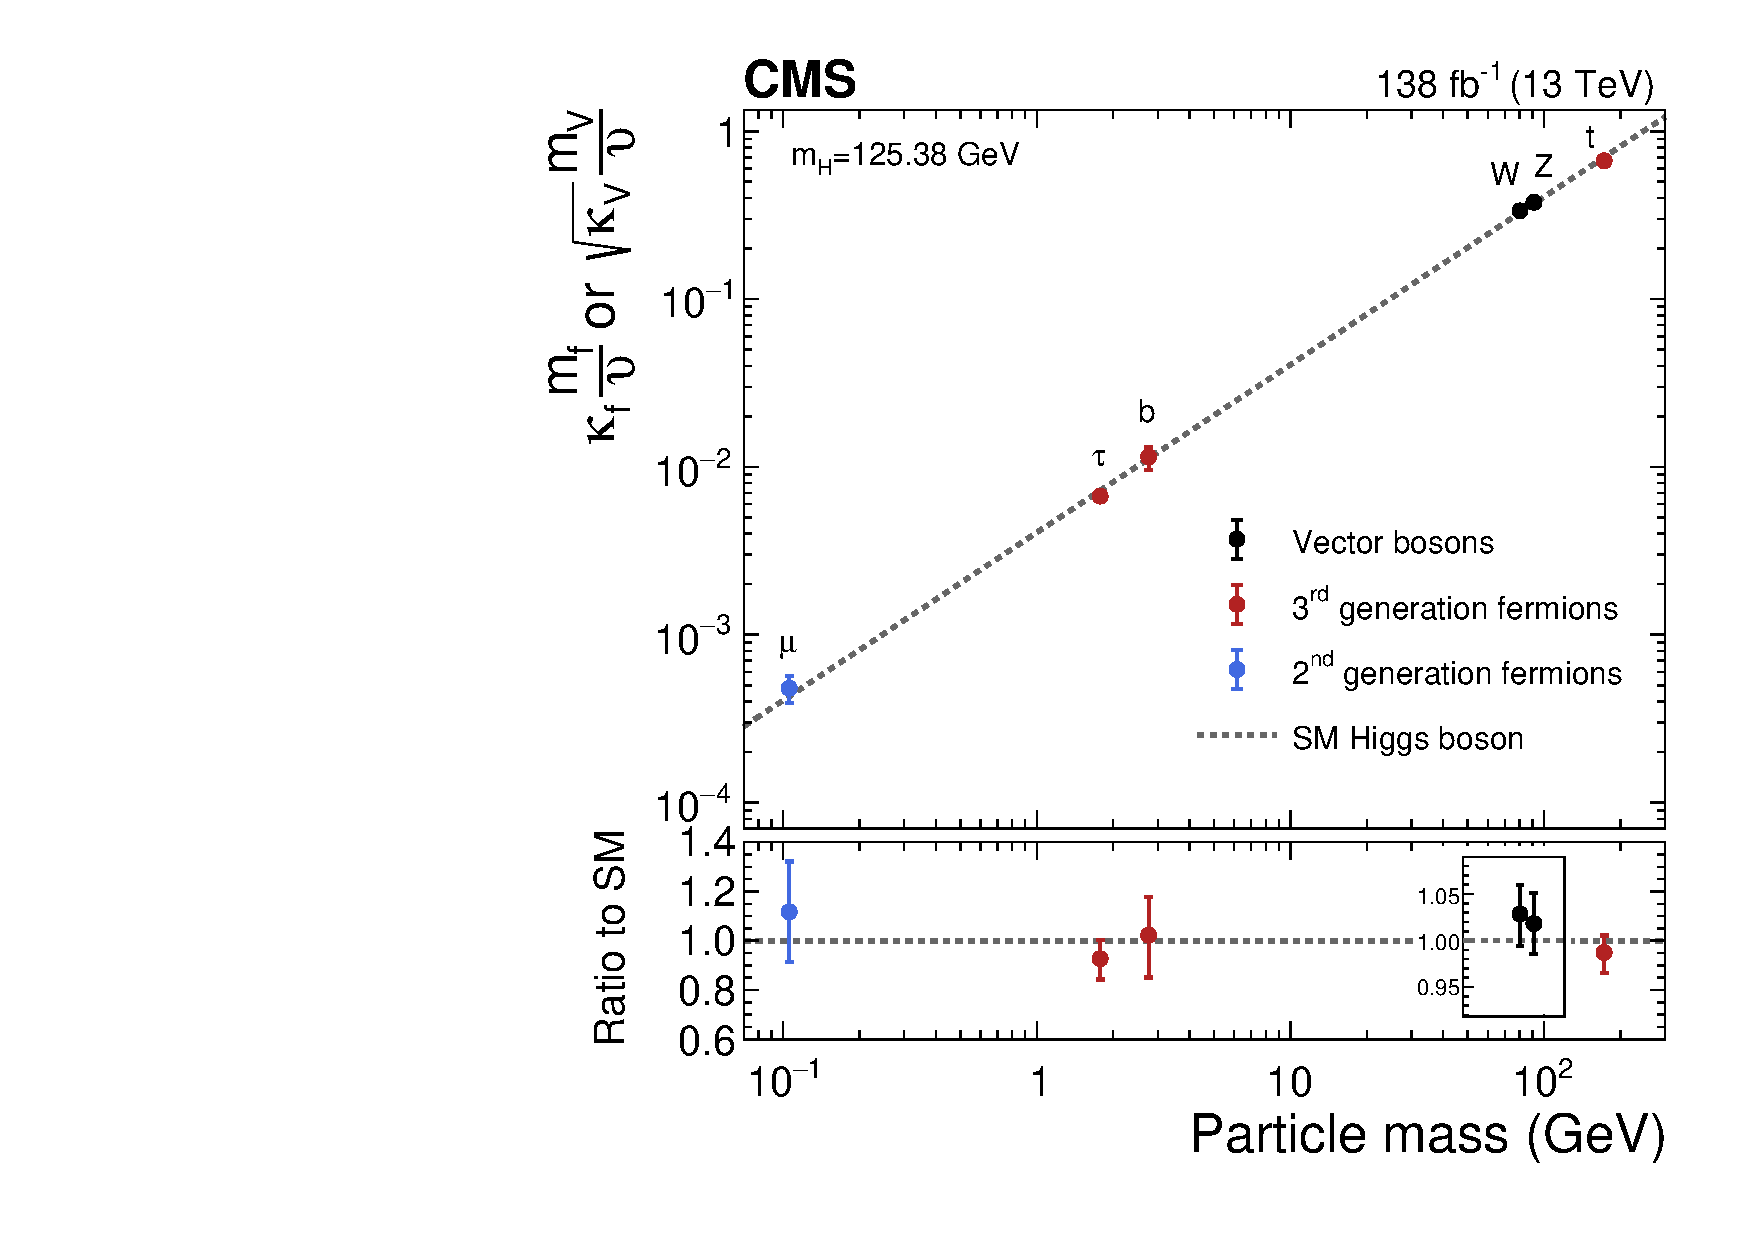
\includegraphics[width =0.65\linewidth]{Figures/Introduction/CMS_couplings_Run2.pdf}\hfill
\caption[Measured couplings of the Higgs boson to vector bosons and fermions.]{A summary of the measured couplings of the Higgs boson to the vector bosons (black markers), third generation fermions (red), and muons (blue). The results are expressed in the coupling modifier $\kappa$-framework~\cite{YR3}, which introduces multiplicative factors at Higgs boson coupling vertices that parameterise deviations from SM behaviour. The error bars represent the 68\% confidence level intervals on the measured parameters. The results are compatible with the SM predictions (dashed line), over four orders of magnitude. Figure taken from Ref~\cite{CMSHiggsNature}. }%For gauge bosons, the square root of the coupling modifier is plotted, to keep a linear proportionality to the mass, as predicted in the SM. The P value with respect to the SM prediction for the right plot is 37.5%.
\label{fig:run_2_couplings}
\end{figure}

%For the \Hee decay, the SM predicted branching fraction is given by:
%\begin{equation}
%    \frac{G_{F}m_{\mathrm{H}}m_{e}^{2}}{4\sqrt{2}\pi\Gamma_{\mathrm{H}}} \approx 5\times10^{-9},
%\end{equation}

%where $m_{H}$ and $\Gamma_{H}$ are the mass and natural width of the Higgs boson respectively, $G_{F}$ is the Fermi constant, and $m_{e}$ is the mass of the electron. 

This thesis studies the extremely rare decay of the Higgs boson to an electron-positron pair (hereafter referred to simply as an \textit{electron pair}), \Hee. The SM predicted branching fraction for this process is extremely small, at around ${\BHee \approx 5.2\times10^{-9}}$; however, a search for \Hee decays provides the only direct probe of the Higgs boson coupling to the electron\footnote{Indirect probes of the electron Yukawa coupling also exist, such as via measurements of the electron electric dipole moment~\cite{ACME}.}. Previously, both the CMS and ATLAS Collaborations have performed searches for \Hee decays. The most sensitive search from CMS was performed using data collected from proton-proton (pp) collisions at a centre-of-mass energy (${\sqrt{s}}$) of 8~TeV, with an integrated luminosity of 19.7~\fbinv. A 95\% confidence level (CL) upper limit on the \Hee branching fraction of approximately ${1.9\times10^{-3}}$ (${3.7 \times 10^{5}}$ times the SM prediction) was determined~\cite{CMSHeeRun1}. The most sensitive limit on \BHee from the ATLAS Collaboration was performed using 139~\fbinv of pp data, collected at ${\sqrt{s}=13}$~TeV, where a 95\% CL upper limit on the branching fraction was set at ${3.6\times10^{-4}}$ (${6.9 \times 10^{4}}$ times the SM prediction)~\cite{ATLASHeeRun2}.
%EMD = requires asymmetric charge distribution along with particles spin. Without CP effects, would require time reveral asymmetry. The electron EDM < 10^-44 in the SM -> non zero means CP violating effects, which in the SM come from CKM and neutrino sectiors, but could be other BSM physics e.g. Higgs physics, super symmetry etc, and the measurements put bounds on the mass scale of these theories. So this measurement can only really probe CP odd contributions to the coupling, coming from loop diagrams involving quarks which are subject to CKM mising and CP violation. Best limit from ACME is 20^-29

The analysis described in this thesis was performed at the CMS experiment using data collected from pp collisions at \sqrts~TeV, and is published in Ref~\cite{HIG-21-015-PAS}. The data were collected during the Run 2 campaign of the LHC between 2016 and 2018, and correspond to an integrated luminosity of \intlumi. In order to improve the analysis sensitivity, event categories are formed to target multiple Higgs boson production modes. Each category is defined using a dedicated machine learning (ML) discriminant trained to separate Higgs boson signal events from background processes. Finally, a simultaneous fit to the dielectron invariant mass distribution (\mee) in each analysis category is used to extract a potential \Hee signal. Given the extremely small expected branching fraction, any observation of the signal process with the current dataset available from the LHC would constitute evidence for physics beyond the SM.

The remainder of this thesis is structured as follows. Chapter~\ref{chap:theory} describes the structure of the SM as a gauge field theory, with a particular focus on the BEH mechanism. The phenomenology of the Higgs boson at the LHC is also discussed. Chapter~\ref{chap:machineLearning} provides an overview in the field of ML. The aim of this chapter is to contextualise the methods and models explored in other chapters of this thesis. The components of the LHC and CMS detector are described in chapter~\ref{chap:detector}. This includes the CMS calorimeter endcap upgrade project (HGCAL), where emphasis is placed on ML models used within the first level of event triggering. Chapter~\ref{chap:objectReco} describes how events recorded with the CMS detector are reconstructed. The particle candidates used in the \Hee search are presented, with emphasis placed on the reconstruction and identification of electrons. The categorisation targeting \Hee events is presented in chapter~\ref{chap:eventCategorisation}, with a focus on the ML techniques used to reject background events. Chapter~\ref{chap:s_b_modelling} outlines the signal and background models used to describe the dielectron mass distribution in each analysis category. Systematic uncertainties considered in the analysis are also discussed. Chapter~\ref{chap:results} describes the statistical methods used to extract the results of the analysis. The expected and observed upper limits on the \Hee branching fraction are presented. Finally, chapter~\ref{chap:conclusions} summarises the \Hee analysis, and offers a brief outlook on future searches.


